Outro dos objetivos da dissertação é a autenticação com \acrfull{cmd} pelo que é necessário adquirir conhecimento sobre o Autenticação.gov.
Este autenticação irá permitir que os utilizadores se autentiquem na plataforma da \acrshort{clav} com recurso ao seu número telemóvel,
\acrshort{pin} da \acrshort{cmd} e \acrshort{pin} temporário enviado por \acrshort{sms} ao número de telemóvel. Para um utilizador poder
usar esta forma de autenticação necessita de ativar a \acrshort{cmd} no Autenticação.gov criando um \acrshort{pin} da \acrshort{cmd}.

De seguida, é aprofundado o Autenticação.gov essencial para permitir esta forma de autenticação.

\section{Estado da Arte}

\subsection{Autenticação.gov}
O Autenticação.gov surgiu da necessidade de identificação unívoca de um utilizador perante sítios na 
Web.~\cite{agov} Será este componente a realizar o processo de autenticação do utilizador e a fornecer
 os atributos do utilizador necessários para identificar o utilizador numa entidade (\textit{website}/portal).

O \acrshort{cc} em conjunto com o Autenticação.gov permite obter os identificadores dos utilizadores junto das 
entidades participantes da iniciativa do \acrshort{cc} (funcionalidade de Federação de Identidades da Plataforma 
de Interoperabilidade da Administração Pública). Além disso, o Autenticação.gov gere os vários fornecedores de 
atributos disponíveis bem como possui uma estreita ligação com a infraestrutura de chave pública do \acrlong{cc} 
(\acrfull{pki}), com o intuito de manter os elevados níveis de segurança e privacidade no processo de autenticação 
e identificação.~\cite{agov}

O Autenticação.gov permite também a criação de credenciais comuns a todos os sites da \acrshort{ap}, ou seja, 
o utilizador apenas necessita de se autenticar uma vez que poderá aceder aos vários portais (Portal do Cidadão, 
etc) com a mesma autenticação (\acrshort{sso}).

Para além disso o utilizador pode autenticar-se utilizando outros certificados digitais que não o \acrshort{cc} 
(por exemplo \acrfull{cmd}, \textit{user+password} ou redes sociais, estes dois últimos quando o 
\textit{website}/portal necessita apenas de conhecer do utilizador o \textit{email}).

No projeto \acrshort{clav} irá ser implementado a autenticação com recurso ao Autenticação.gov através de dois 
certificados digitais diferentes:
\begin{itemize}
    \item \acrfull{cc}: Já se encontra implementado como referido na secção~\ref{sec:autenticacao}. 
    A autenticação é realizada através da leitura do \acrshort{cc} (através de um leitor de cartões sendo 
    necessário a instalação de \textit{software} do Autenticação.gov para proceder à leitura do \acrshort{cc}) e 
    posterior inserção do \acrshort{pin} de autenticação recebido quando se cria/renova o \acrshort{cc};

    \item \acrfull{cmd}: Um dos objetivos desta tese é a implementação da autenticação com recurso a este 
    certificado digital. Com a \acrshort{cmd}, após o utilizador associar um número de telemóvel ao 
    \acrshort{nic}, o utilizador pode autenticar-se com o número de telemóvel, o código \acrshort{pin} da 
    \acrshort{cmd} e o código de segurança temporário enviado por \acrshort{sms}.
\end{itemize}

De forma a completar a figura~\ref{fig:authgov} apresenta-se de seguida, na figura~\ref{fig:fluxoauthgov}, o fluxo de pedidos efetuado entre 
a \acrshort{clav} e o Autenticação.gov de forma a autenticar um utilizador na \acrshort{clav}:~\cite{agov}
\begin{figure}[H]
    \centering
    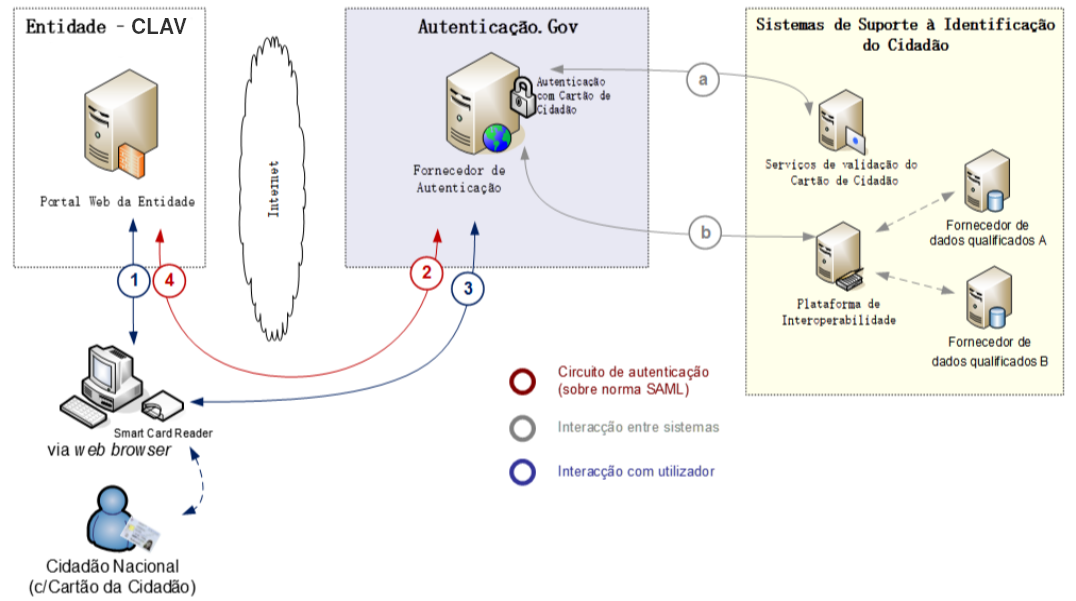
\includegraphics[width=1\textwidth]{img/fluxoauthgov.png}
    \caption{Fluxo de pedidos entre a \acrshort{clav} e o Autenticação.gov de forma a autenticar um utilizador na \acrshort{clav}.~\cite{agov}}\label{fig:fluxoauthgov}
\end{figure}

\begin{enumerate}
    \item O utilizador pretende aceder à área privada do portal de uma entidade (da \acrshort{clav}), na qual 
    é necessário que comprove a sua identidade;
    \item O portal da entidade (\acrshort{clav}) delega a autenticação e redireciona o utilizador para o 
    Autenticação.gov, juntamente com um pedido de autenticação assinado digitalmente;
    \item O Autenticação.gov valida o pedido de autenticação recebido e solicita a autenticação do utilizador 
    com recurso ao seu \acrshort{cc} pedindo a inserção do seu \acrshort{pin} de autenticação. 
    Durante este processo, o Autenticação.gov efetua as seguintes operações internas:
    \begin{enumerate}
        \item Valida as credenciais do utilizador com recurso à \acrshort{pki} do \acrshort{cc} 
        via \acrshort{ocsp};
        \item Obtém atributos que sejam solicitados pelo portal da entidade (\acrshort{clav}) junto dos vários 
        fornecedores de atributos qualificados. Esta operação é efetuada via Plataforma de Interoperabilidade. 
        Este processo pode incluir a obtenção de dados da Federação de Identidades ou de outras Entidades.
    \end{enumerate}

    \item A identificação e atributos do utilizador são autenticados e assinados digitalmente pelo 
    Autenticação.gov, após o qual redireciona o utilizador de volta ao portal da entidade original (\acrshort{clav}). Cabe à entidade (\acrshort{clav}) a validação das credenciais do Autenticação.gov e utilização dos atributos do cidadão.
\end{enumerate}

A troca de pedidos entre a \acrshort{clav} e o Autenticação.gov é feita através de \acrshort{saml} 2.0.

O \acrfull{saml} define uma \textit{framework} \textit{standard} em \acrshort{xml}.~\cite{sam2man} 
Foi aprovado pela \acrshort{oasis}, permite a troca segura de informação de autenticação e autorização entre 
diferentes entidades possibilitando através de uma credencial (\textit{login} de um utilizador) aceder autenticado 
a um conjunto de \textit{websites} (\acrshort{sso}).

Para utilizar o Autenticação.gov é necessário criar um pedido baseado em \acrshort{saml}, assinado digitalmente 
com um certificado X.509 (permite ao Autenticação.gov identificar a entidade responsável pelo pedido) e encriptado 
com a chave privada de um par de chaves \acrshort{rsa} (permite ao Autenticação.gov verificar a validade do 
pedido de autenticação), bem como a respetiva cadeia de autenticação.~\cite{otavioTese} 
A chave pública do par de chaves \acrshort{rsa} faz parte do certificado X.509 que é enviado ao Autenticação.gov.

Há dois tipos de \acrshort{saml} usados com o Autenticação.gov~\cite{otavioTese}:
\begin{itemize}
    \item \textbf{\acrshort{saml} Request (2 da figura~\ref{fig:fluxoauthgov}):} Pedido de autenticação, 
    enviado ao Autenticação.gov, no qual é enviado a origem, assinaturas, atributos a obter do utilizador, etc.
    \item \textbf{\acrshort{saml} Response (4 da figura~\ref{fig:fluxoauthgov}):} Resposta ao pedido de 
    autenticação enviado para o \textit{issuer} do pedido de autenticação. Esta resposta contém o 
    \textit{status} do pedido de autenticação (sucesso, insucesso ou cancelado) e no caso de uma autenticação 
    com sucesso contém os atributos do utilizador requisitados.
\end{itemize}

Tanto o pedido e a resposta estão no formato \acrshort{xml} pelo simples facto de ser usado o \acrshort{saml} 2.0.

No caso do \textit{\acrshort{saml} Request} o pedido possui o elemento \textit{root} \texttt{AuthnRequest} onde 
se destacam os seguintes atributos:
\begin{itemize}
    \item \textbf{Destination}: \acrshort{url} para o qual o pedido de autenticação é enviado. No caso da 
    Autenticação.gov este apenas pode ser um dos seguintes \acrshort{url}'s:
    \begin{itemize}
        \item \url{https://preprod.autenticacao.gov.pt/fa/Default.aspx} para o ambiente de teste;
        \item \url{https://autenticacao.gov.pt/fa/Default.aspx} para o ambiente de produção 
        (obrigatório o uso de \acrshort{https} para a comunicação).
    \end{itemize}
    \item \textbf{AssertionConsumerServiceURL}: \acrshort{url} destino da resposta do pedido de autenticação 
    (\textit{\acrshort{saml} Response}). Em produção, é obrigatório que o \acrshort{url} seja em \acrshort{https};
    \item \textbf{ProviderName}: Nome da plataforma/aplicação que está a requerer a autenticação através do 
    Autenticação.gov. Este nome tem de ser previamente acordado com a \acrshort{ama} durante a emissão da cadeia 
    de autenticação e certificados X.509~\cite{otavioTese}.
\end{itemize}

Além destes atributos, o \textit{\acrshort{saml} Request} possui 3 elementos aninhados:\label{sec:soaAuthCMDReq}
\begin{itemize}
    \item \textbf{Issuer}: Informação sobre quem efetua o pedido de autenticação, ou seja a \acrshort{clav}. 
    Basta apenas enviar o \acrshort{url} de onde é originário o pedido;
    \item \textbf{Signature}: Assinatura digital do pedido. Aqui é adicionado o certificado X.509 com a cadeia de 
    autenticação fornecida pela \acrshort{ama};
    \item \textbf{Extensions}: Contém os atributos a requisitar ao Autenticação.gov do utilizador a autenticar-se 
    na \acrshort{clav}. Aqui são também adicionados o nível de confiança e a política de apresentação do 
    Autenticação.gov:
    \begin{itemize}
        \item \textbf{Nível de confiança} \\
        Permite indicar o nível mínimo necessário para realizar a autenticação. Os níveis passíveis de usar 
        são~\cite{agov2}:
        \begin{itemize}
            \item 4:
            \begin{itemize}
                \item Autenticação com recurso a uma ou mais operações criptográficas efetuadas no \acrlong{cc} 
                em autenticação que resulta num conjunto de informação fornecida ao Autenticação.gov que permite 
                com o maior grau de certeza de que, no momento da autenticação, se utilizou um \acrlong{cc} real 
                com conhecimento do \acrshort{pin} de autenticação;
                \item Autenticação com renegociação \acrshort{ssl} com certificado cliente da Ordem dos Notários, 
                da Ordem dos Advogados ou da Câmara dos Solicitadores;
            \end{itemize}
            \item 3: Autenticação com \acrlong{cmd};
            \item 2: Autenticação com \acrlong{cmd} através de Email ou \textit{Twitter};
            \item 1: Autenticação com Utilizador/Palavra-passe (também designado por Autenticação Simples) e 
            Redes Sociais.
        \end{itemize}
        \item \textbf{Política de apresentação} \\
        No Autenticação.gov quando o nível de confiança é inferior a 4 são apresentadas múltiplas abas com os 
        Mecanismos de Autenticação disponíveis. A política de apresentação permite definir o que deve ou não ser 
        apresentado (que abas devem estar disponíveis tendo em conta o nível de confiança definido) e/ou que 
        método de autenticação (aba) deve ser o predefinido. Em caso de conflitos entre o nível de confiança e a 
        política de apresentação ou conflitos na própria política de apresentação, esta é ignorada e é utilizada 
        a política de apresentação que privilegia o \acrshort{cc} (mecanismo de autenticação mais seguro). 
        Os Mecanismos de Autenticação disponíveis são~\cite{agov2}:
            \begin{itemize}
                \item \acrlong{cc};
                \item \acrlong{cmd};
                \item Utilizador/Palavra-passe também designado por Autenticação Simples;
                \item Redes Sociais.
            \end{itemize}
            E o mapeamento das abas aos mecanismos de autenticação é~\cite{agov2}:
            \begin{itemize}
                \item 'CC': Aba relativa à autenticação através de \acrlong{cc};
                \item 'CMD': Aba relativa à autenticação através de \acrlong{cmd};
                \item 'UPP': Aba relativa à autenticação através de Utilizador/Palavra-passe;
                \item 'RSS': Aba relativa à autenticação através das Redes Sociais.
            \end{itemize}
            Esta identificação é usada para identificar as abas na extensão em XML.
    \end{itemize}
\end{itemize}

Após a receção do \textit{\acrshort{saml} Request}, o Autenticação.gov processa a autenticação do utilizador 
e retorna o \textit{\acrshort{saml} Response} como resposta.

O \textit{\acrshort{saml} Response} tem como elemento \textit{root} \textit{Response}.
Este elemento possui 5 elementos aninhados dos quais se destaca:
\begin{itemize}
    \item \textbf{Status}: Contém a informação relativa ao sucesso ou insucesso do pedido de autenticação;
    \item \textbf{Assertion}: Asserção \acrshort{saml} que contém os atributos requisitados sobre o utilizador 
    no caso do pedido de autenticação ter sucesso.
\end{itemize}

Para finalizar é importante referir que o Autenticação.gov é como se fosse uma caixa negra à qual é enviado um 
pedido pela entidade que necessita a autenticação do utilizador (neste caso a \acrshort{clav}) com algumas 
configurações a usar pelo Autenticação.gov e, esta caixa negra, devolve a informação do utilizador autenticado 
(os atributos do utilizador requisitados no pedido efetuado ao Autenticação.gov). Os atributos são apenas 
devolvidos à entidade caso o utilizador autorize o Autenticação.gov a dar à entidade essa informação. 
A caixa negra trata de autenticar o utilizador através das credenciais fornecidas por este.

Para um maior aprofundamento sobre o Autenticação.gov recomenda-se a leitura da secção 2.2 da 
dissertação~\cite{otavioTese} (``CLAV: Autenticação e integração na plataforma iAP'' de Octávio Maia).

\section{Solução}

A autenticação com \acrshort{cmd} é bastante semelhante à autenticação com o \acrshort{cc}. 
O que muda é o modo de autenticação perante o Autenticação.gov que em vez de ser efetuado com \acrshort{cc} 
(\acrlong{cc}, Leitor de Cartões, \textit{software} local do Autenticação.gov e \acrshort{pin} de autenticação 
do \acrshort{cc}) será realizado através de \acrshort{cmd} (Número de telemóvel, \acrshort{pin} definido durante 
a ativação da \acrshort{cmd} e \acrshort{pin} temporário enviado para o número de telemóvel).

Os atributos pedidos ao Autenticação.gov são os mesmos que são pedidos com a autenticação com o \acrshort{cc} 
(\acrshort{nic} e Nome Completo) permitindo identificar unicamente o utilizador a partir do \acrshort{nic}. 
Para além disso, permite aproveitar todo o back-end e código já desenvolvido para a autenticação do utilizador 
perante a \acrshort{clav} através de \acrshort{cc} visto que os atributos usados são os mesmos. 
Além disso, permite uma melhor normalização da identificação dos utilizadores (não existindo assim vários ids 
para o mesmo utilizador) bem como evita ser necessário o utilizador partilhar atributos adicionais (como o 
número de telemóvel) com a \acrshort{clav} (o número de telemóvel é apenas partilhado com o Autenticação.gov 
sendo que a \acrshort{clav} não tem acesso a esta informação se apenas pediu para saber os atributos 
\acrshort{nic} e Nome Completo). Assim, a única implicação que pode ser retirada daqui é que o utilizador, 
quer queira usar a autenticação por \acrshort{cc} quer queira usar por \acrshort{cmd}, necessita de estar 
registado na \acrshort{clav} com o \acrshort{cc} sendo que, neste momento é obrigatório o registo dos utilizadores 
através de \acrshort{cc}. 

Volta-se a frisar que o \acrshort{nic} será usado por forma a identificar o utilizador, 
pelo que serve de id do utilizador tal como na autenticação com o \acrshort{cc}.

Portanto, de igual forma como na autenticação com o \acrshort{cc}, quando é selecionado este método de autenticação,
 a \acrshort{clav} redireciona o utilizador para o Autenticação.gov que se encarrega de autenticar o utilizador 
 com \acrshort{cmd}, comunicando, no fim, os atributos pedidos ao Autenticação.gov (\acrshort{nic} e Nome Completo).
  A \acrshort{clav} com o \acrshort{nic} verifica se o utilizador já se encontra registado, obtendo mais alguma 
  informação adicional, como o nível de utilizador. 
  
  Semelhantemente à autenticação local e à autenticação com o \acrshort{cc}, é agora gerado um \textit{token} 
  (\acrshort{jwt}) que irá assinar a partir daqui todos os pedidos do utilizador. O \textit{token} tem a validade 
  de 8 horas, ao fim das quais o utilizador necessita de realizar uma nova autenticação.

Em termos técnicos, é apenas necessário aproveitar o pedido POST que já é enviado ao Autenticação.gov para a 
autenticação com \acrshort{cc} e adicionar as extensões nível de confiança e a política de apresentação como 
é possível constatar em~\ref{sec:soaAuthCMDReq}.

A primeira extensão permite indicar o nível mínimo necessário que pretendemos que seja usado pelo Autenticação.gov. 
Como tal, dado um nível selecionado permite a autenticação através do método desse nível mas também permite os 
métodos de autenticação dos níveis superiores. Além disso, quanto menor o nível mais fraca é a autenticação, 
visto que quanto menor o nível mais fraca é a autenticidade das credenciais fornecidas pelo utilizador.

Quando este nível de confiança não está presente (como no caso do pedido enviado para a autenticação 
com \acrshort{cc}) o nível de confiança mínimo assumido é o nível máximo (4). Assim para o caso da \acrshort{cmd} 
será adicionada a seguinte extensão ao pedido em XML~\cite{agov2}:
%Ref: Manual de Integração do Fornecedor de Autenticação v1.5.3 cap 7.2
\begin{lstlisting}[language=xml, caption=Extensão Nível de Confiança no pedido enviado ao Autenticação.gov]
<fa:FAAALevel xmlns:fa="http://autenticacao.cartaodecidadao.pt/atributos">
    3
</fa:FAAALevel>
\end{lstlisting}

Esta extensão indica então que o nível de confiança mínimo necessário é o nível 3, ou seja, permite a autenticação 
através de \acrshort{cmd} mas também através de \acrshort{cc}.

Como tal, por forma a apenas aparecer no Autenticação.gov a hipótese de autenticação através de \acrshort{cmd} é 
necessário definir a Política de Apresentação do Autenticação.gov.

Ou seja, é necessário esconder a aba do \acrfull{cc} e se futuramente se pretender apresentar ambas as abas é 
também necessário tornar o mecanismo de \acrfull{cmd} a aba predefinida. Para tal, foi adicionada a seguinte 
extensão ao pedido em XML~\cite{agov2}:
%Ref: Manual de Integração do Fornecedor de Autenticação v1.5.3 cap 8.2
\begin{lstlisting}[language=xml, caption=Extensão Política de Apresentação no pedido enviado ao Autenticação.gov]
<fa:AuthTabPresentationPolicies xmlns:fa="http://autenticacao.cartaodecidadao.pt/presentationpolicy">
    <!--Torna a aba CMD como predefinida-->
    <fa:defaultSelectedAuthTab TabId="CMD"/>
    <!--Esconde a aba do CC-->
    <fa:hideAuthTab TabId="CC"/> 
</fa:AuthTabPresentationPolicies>
\end{lstlisting}

Que torna a aba do mecanismo de \acrshort{cmd} o predefinido e esconde a aba do mecanismo de \acrshort{cc}.

Portanto, se for enviado um pedido ao Autenticação.gov igual ao da autenticação com \acrshort{cc} mas com estas 
extensões, o Autenticação.gov pedirá ao utilizador para se autenticar com \acrshort{cmd}.

\section{Implementação}

Nesta secção será demonstrado como se pode utilizar esta forma de autenticação através da interface da \acrshort{clav}. Para iniciar o processo o utilizador deve aceder a \url{https://clav.dglab.gov.pt/users/autenticacao} e carregar no botão ``Chave Móvel Digital''. Após carregar no botão, o utilizador é redirecionado para o Autenticação.gov onde lhe é apresentada uma página a pedir autorização para a partilha do Nome Completo e do \acrshort{nic} do utilizador com a \acrshort{clav} como se pode observar na figura~\ref{fig:CMDauto}. O utilizador ao autorizar, aparece-lhe o formulário para a inserção do número de telemóvel e do \acrshort{pin} da \acrshort{cmd} como presente na figura~\ref{fig:CMDcreds}. Após carregar em ``Autenticar'' se os valores estiverem corretos aparecerá o formulário para introduzir o \acrshort{pin} temporário enviado por \acrshort{sms} como se observa na figura~\ref{fig:CMDcredTemp}.

\begin{figure}[H]
    \centering
    \begin{subfigure}{.32\textwidth}
        \centering
        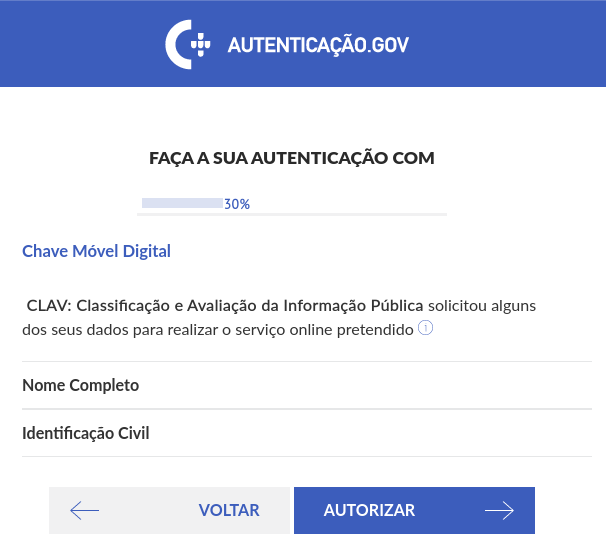
\includegraphics[width=1\linewidth]{img/CMDauto.png}
        \caption{Pedido de autorização para partilha de atributos\label{fig:CMDauto}}
    \end{subfigure}
    \begin{subfigure}{.32\textwidth}
        \centering
        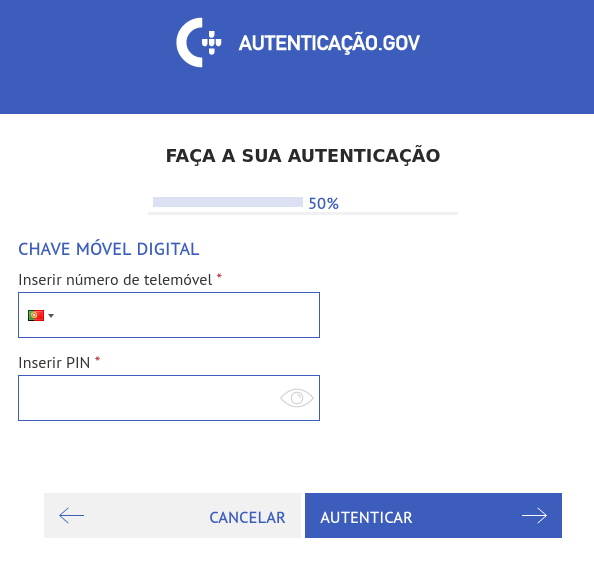
\includegraphics[width=1\linewidth]{img/CMDcreds.png}
        \caption{Formulário da \acrshort{cmd}\label{fig:CMDcreds}}
    \end{subfigure}
    \begin{subfigure}{.32\textwidth}
        \centering
        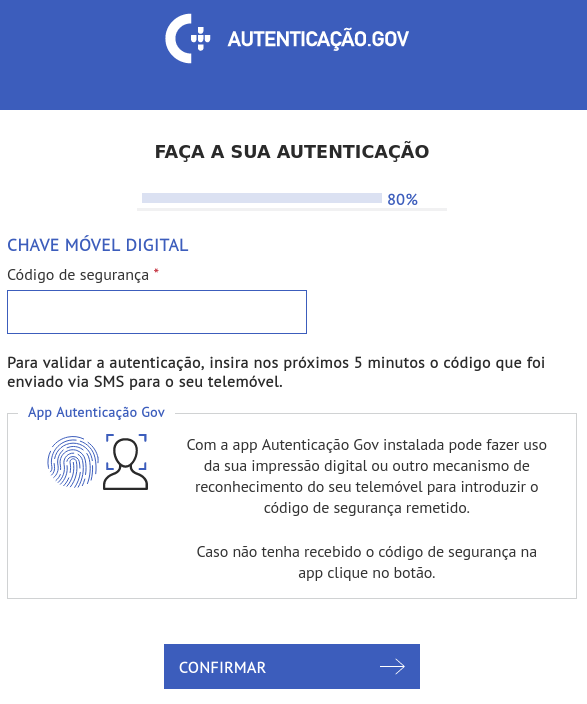
\includegraphics[width=1\linewidth]{img/CMDcredTemp.png}
        \caption{Formulário do \acrshort{pin} temporário da \acrshort{cmd}\label{fig:CMDcredTemp}}
    \end{subfigure}
    \caption{Autenticação.gov: Processo de autenticação com \acrshort{cmd}}
\end{figure}

Ao fim de carregar em ``Confirmar'' e caso o \acrshort{pin} temporário esteja correto, o utilizador é redirecionado de volta para a \acrshort{clav} onde aparecerá ao utilizador uma de duas hipóteses:
\begin{itemize}
    \item Se o utilizador já se encontra registado na \acrshort{clav} então autentica-se com sucesso onde é redirecionado para a \textit{Home Page} da \acrshort{clav} como se observa na figura~\ref{fig:CMDauthSuc}:
    \begin{figure}[H]
        \centering
        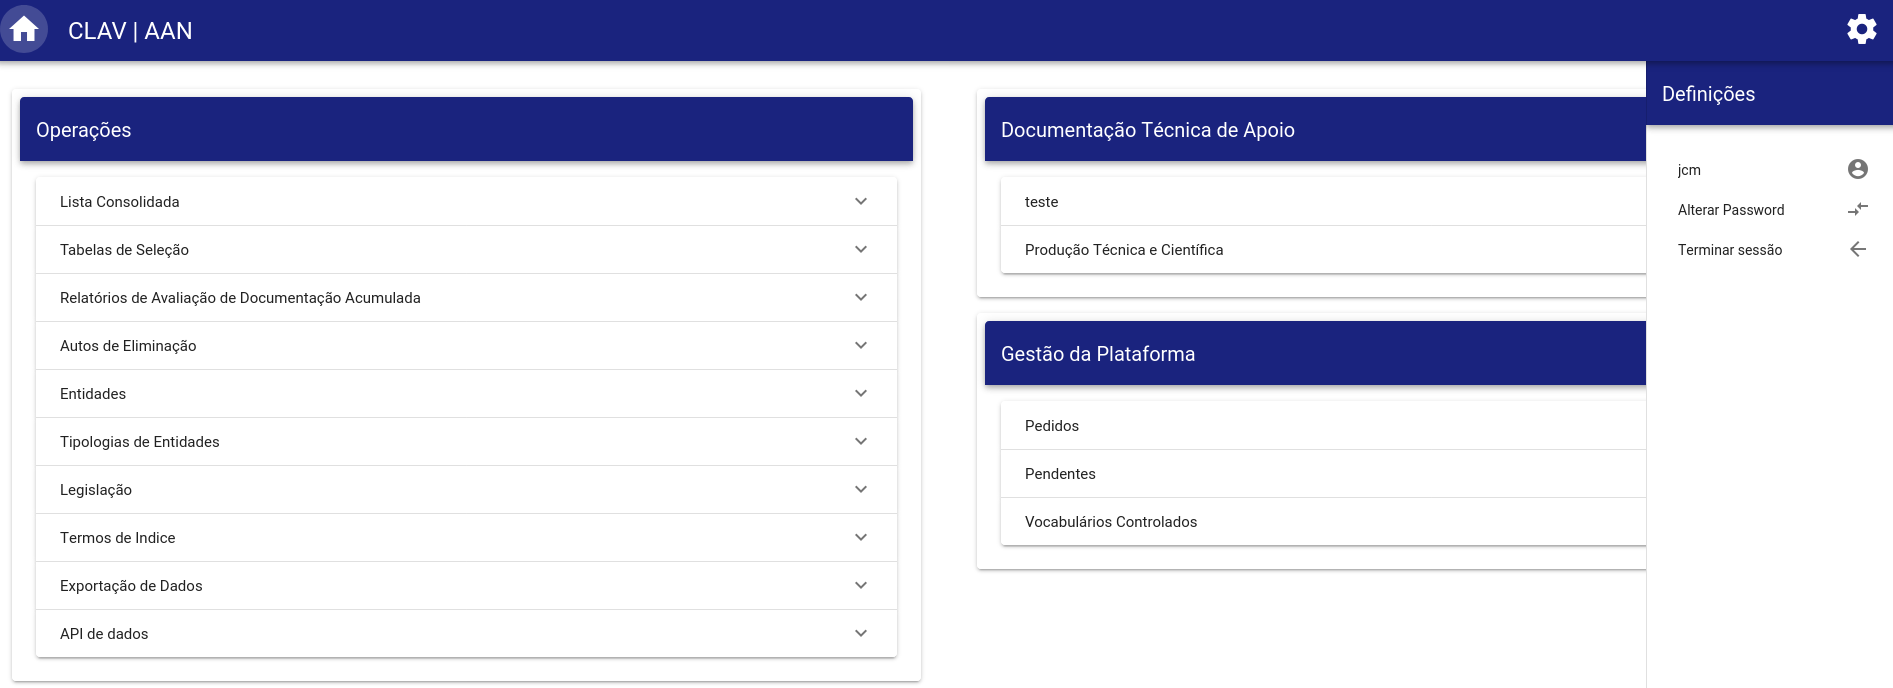
\includegraphics[width=0.5\textwidth]{img/CMDauthSuc.png}
        \caption{Utilizador autenticado com sucesso através de \acrshort{cmd}\label{fig:CMDauthSuc}}
    \end{figure}
    \item Se o utilizador ainda não se encontra registado na \acrshort{clav} então não é autenticado na \acrshort{clav} apresentando uma mensagem de erro como na figura~\ref{fig:CMDnotReg}:
    \begin{figure}[H]
        \centering
        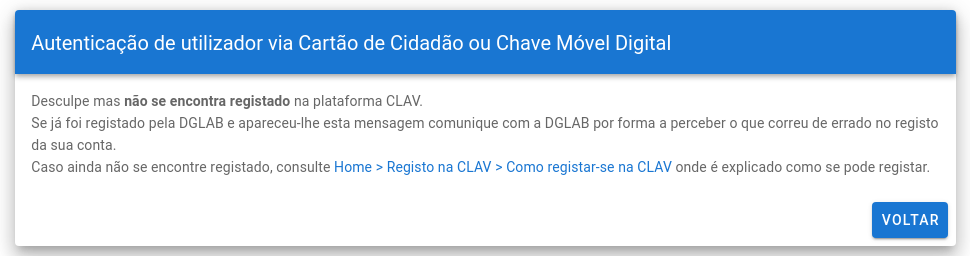
\includegraphics[width=0.5\textwidth]{img/CMDnotReg.png}
        \caption{Mensagem de erro na \acrshort{clav} caso não se encontre registado na \acrshort{clav} mas tenha se autenticado com sucesso no Autenticação.gov\label{fig:CMDnotReg}}
    \end{figure}
\end{itemize}

Por fim, caso o utilizador cancele algum dos passos de autenticação do Autenticação.gov, se engane em alguma credencial ou aconteça algum erro no Autenticação.gov é redirecionado de volta para a \acrshort{clav} onde lhe é apresentado a mensagem de erro presente na figura~\ref{fig:CMDerror}:

\begin{figure}[H]
    \centering
    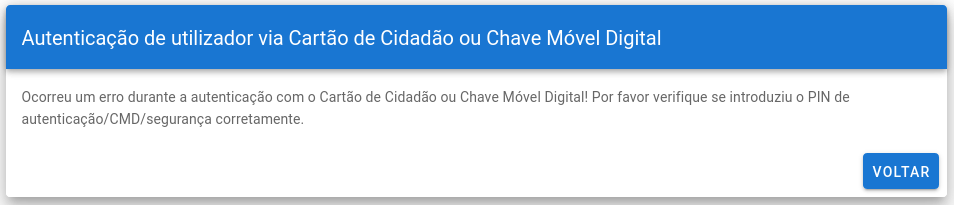
\includegraphics[width=0.5\textwidth]{img/CMDerror.png}
    \caption{Mensagem de erro na \acrshort{clav} após falha no Autenticação.gov\label{fig:CMDerror}}
\end{figure}

\section{Resumo}

Após um breve aprofundamento do Autenticação.gov foi descrita a solução desenvolvida e na secção da implementação apresentou-se o processo de autenticação através de \acrlong{cmd} presente.
